\subsubsection{Data}
We have generated the data for the regression problem using the Franke function \citep[p. 13]{frank}.
\begin{align}
\begin{split}\label{eq:franke}
    f(x, y) = &\frac{3}{4} \exp\left( -\frac{(9x - 2)^2}{4} - \frac{(9y - 2)^2}{4} \right) \\
    + &\frac{3}{4} \exp\left( -\frac{(9x + 1)^2}{49} - \frac{(9y + 1)^2}{10} \right)  \\
    + &\frac{1}{2} \exp\left( -\frac{(9x - 7)^2}{4} - \frac{(9y - 3)^2}{4} \right)  \\
    - &\frac{1}{5} \exp\left( -(9x - 4)^2 - (9y - 7)^2 \right),
\end{split}
\end{align}
\begin{align}\label{eq:franke_noise}
    f^*(x,y) = f(x, y) + \frac{\gaute{3}}{10} \mathcal{N}(0, 1),
\end{align}
The Franke function is defined by Eq. \ref{eq:franke}, on the domain $[0, 1]^2$. 
In order to challenge the models, and testing them for weaknesses such as overfitting, we have added a stochastic noise term to the function, as can be seen in Eq. \ref{eq:franke_noise}.



\begin{figure}[h!]
\centering
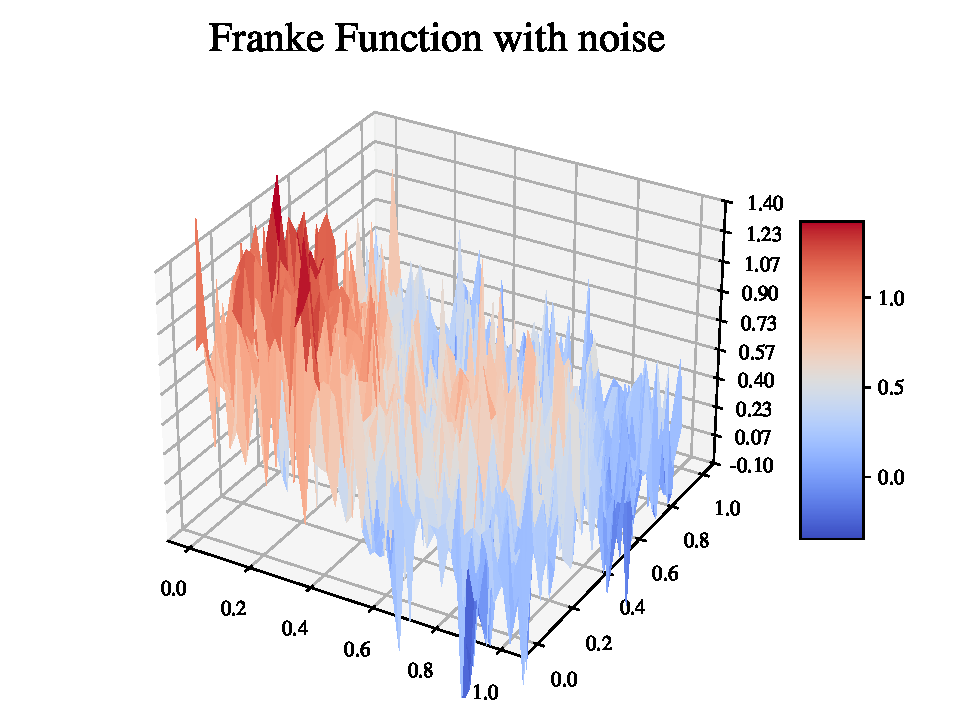
\includegraphics[width=1\linewidth]{project_1/figures/figures_in_report/franke_func_noise.pdf}
\caption{The Franke function for x,y $\in [0,1]$ with added noise term: $(\gaute{3}/10) \mathcal{N}(0, 1)$.} \gaute{update noise if needed}
\label{fig:franke_noise}
\end{figure}

\gaute{In order to enable potential overfitting in the models, we added a stochastic noise term to the Franke function. The noise term is generated using a normal distribution, and scaled by a factor of $0.3$. By choosing this noise term factor, we introduce sufficient amounts of noise to observe overfitting in some models, while maintaining the underlying structure to be recognized by the models (see Fig. \ref{fig:franke_noise}). Hence, we use the following function in our analysis:
where $f(x,y)$ is defined in Eq. \ref{eq:franke}. All mentions of the Franke function henceforth will reference the function defined in Eq. \ref{eq:franke_noise}.
For the Franke data, we use 41 data points along each axis, for a total of 1681 data point (i.e. $41^2$).}

\subsubsection{Linear regression}

\subsubsection{Logistic regression}

\subsubsection{Exploration of the properties of a neural network}

For the classification case, i.e. the Cancer data, we used Binary cross entropy as our \mia{cost eller loss} function. For the Franke function data, the choice was mean squared error (MSE). 

As measures of performance, $R^2$ is used for the Franke function data. 
Furthermore, accuracy, recall, precision and \mia{check this later} is used for the other data set. 

Sigmoid is always utilized as the activation function in the final layer for the classification. 
In the other data set, we do not apply any activation function. 

\julie{should mention that we have chosen to not use specialized initialization methods for bias/weights, bc were testing different network architectures so it doesnt make sense to do + we have small NN so they'll converge quickly anyways.}

In order to explore the properties of the different aspects of our neural network, we \mia{...}

Firstly, we wanted to find a good optimizer to use for the exploration of the other moments. 
We initialized our neural network model with a learning rate of 0.005 and two hidden layers of size 4 and 8 respectively. 
Both the hidden layers had ReLU as the activation function. 
For the Cancer data, sigmoid was used at the final layer, whereas for the Franke function data, we did not use an activation (i.e. identity). 
Furthermore, we used a batch size of 200 and 1000 for the Cancer data and the Franke function data respectively. 

We used all six optimizers and trained six different models for each of the two different data sets. 
We chose the optimizer that performed best for use in further explorations of the neural network. 


\mia{JAX will replace our analytical gradient}

optimizers = ["Constant", "Momentum", "Adam", "Adagrad_Momentum", "RMSprop"]
layer_sizes = [8,16]
num_hidden_layers = [2, 3]
learning_rates = [0.01, 0.001, 0.0001]
batch_sizes_cont = [1000,3000, 5000]
batch_sizes_disc = [100,200, 300]
activation_functions = ["ReLU","sigmoid","leaky_ReLU"]